\documentclass{scrartcl}

\usepackage{lmodern}

\usepackage{tikz}
\usetikzlibrary{automata,positioning}

\begin{document}
  \tableofcontents
  
  \section{Der Reguläre Ausdruck \texttt{|a}}
  
  Initialer Zustand:

  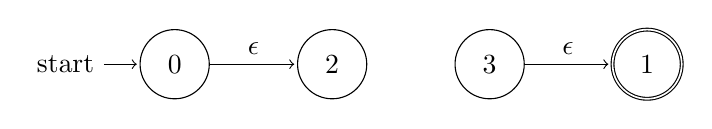
\begin{tikzpicture}[shorten >=1pt,node distance=2cm,on grid,auto]
    \node[state,initial]   (q0)               {$0$};
    \node[state]           (q2) [right=of q0] {$2$};
    \node[state]           (q3) [right=of q2] {$3$};
    \node[state,accepting] (q1) [right=of q3] {$1$};
    
    \path[->] (q0) edge node {$\epsilon$} (q2)
              (q3) edge node {$\epsilon$} (q1);
  \end{tikzpicture}
  
  Der Reguläre Ausdruck \verb!|a! wird eingefügt in zwei Schritten. Der erste Schritt fügt die linke Regel wischen die Knoten $2$ und $3$ ein. Die linke Regel lautet $\epsilon$, und führt daher u folgendem Automaten:
  
  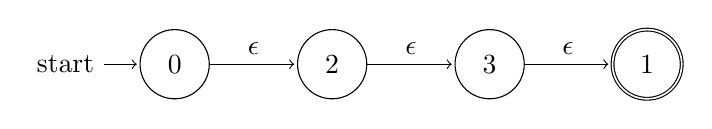
\begin{tikzpicture}[shorten >=1pt,node distance=2cm,on grid,auto]
  \node[state,initial]   (q0)               {$0$};
  \node[state]           (q2) [right=of q0] {$2$};
  \node[state]           (q3) [right=of q2] {$3$};
  \node[state,accepting] (q1) [right=of q3] {$1$};
  
  \path[->] (q0) edge node {$\epsilon$} (q2)
            (q2) edge node {$\epsilon$} (q3)
            (q3) edge node {$\epsilon$} (q1);
  \end{tikzpicture}
  
  Die zweite Regel lautet \verb|a|. Diese wird zuerst gebaut:
  
  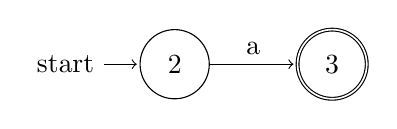
\begin{tikzpicture}[shorten >=1pt,node distance=2cm,on grid,auto]
    \node[state,initial]   (q2)  {$2$};
    \node[state,accepting] (q3) [right=of q2] {$3$};
    
    \path[->] (q2) edge node {a} (q3);
  \end{tikzpicture}
  
  Dieser wird jetzt in den ersten Automaten eingehängt:
  
  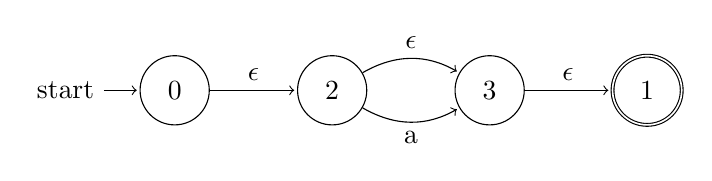
\begin{tikzpicture}[shorten >=1pt,node distance=2cm,on grid,auto]
    \node[state,initial]   (q0)               {$0$};
    \node[state]           (q2) [right=of q0] {$2$};
    \node[state]           (q3) [right=of q2] {$3$};
    \node[state,accepting] (q1) [right=of q3] {$1$};
    
    \path[->] (q0) edge              node         {$\epsilon$} (q2)
              (q2) edge [bend left]  node         {$\epsilon$} (q3)
              (q2) edge [bend right] node [below] {a}          (q3)
              (q3) edge              node         {$\epsilon$} (q1);
    
  \end{tikzpicture}
  
  \section{Der Reguläre Ausdruck \texttt{a|}}
  
  \begin{labeling}[:]{Rechts (kombiniert)}
    \item[Initial] 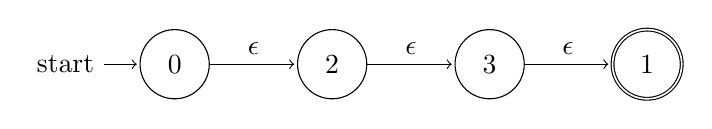
\begin{tikzpicture}[shorten >=1pt,node distance=2cm,on grid,auto]
      \node[state,initial]   (q0)               {$0$};
      \node[state]           (q2) [right=of q0] {$2$};
      \node[state]           (q3) [right=of q2] {$3$};
      \node[state,accepting] (q1) [right=of q3] {$1$};
      
      \path[->] (q0) edge node {$\epsilon$} (q2)
                (q2) edge node {$\epsilon$} (q3)
                (q3) edge node {$\epsilon$} (q1);
    \end{tikzpicture}
    \item[Links] 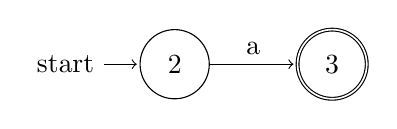
\begin{tikzpicture}[shorten >=1pt,node distance=2cm,on grid,auto]
      \node[state,initial]   (q2)               {$2$};
      \node[state,accepting] (q3) [right=of q2] {$3$};
      
      \path[->] (q2) edge node {a} (q3);
    \end{tikzpicture}
    \item[Kombinieren] 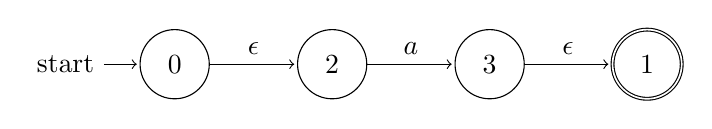
\begin{tikzpicture}[shorten >=1pt,node distance=2cm,on grid,auto]
      \node[state,initial]   (q0)               {$0$};
      \node[state]           (q2) [right=of q0] {$2$};
      \node[state]           (q3) [right=of q2] {$3$};
      \node[state,accepting] (q1) [right=of q3] {$1$};
      
      \path[->] (q0) edge node {$\epsilon$} (q2)
                (q2) edge node {$a$}        (q3)
                (q3) edge node {$\epsilon$} (q1);
    \end{tikzpicture}
    \item[Rechts (kombiniert)] 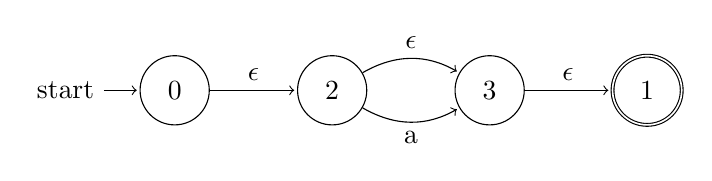
\begin{tikzpicture}[shorten >=1pt,node distance=2cm,on grid,auto]
    \node[state,initial]   (q0)               {$0$};
    \node[state]           (q2) [right=of q0] {$2$};
    \node[state]           (q3) [right=of q2] {$3$};
    \node[state,accepting] (q1) [right=of q3] {$1$};
    
    \path[->] (q0) edge              node         {$\epsilon$} (q2)
              (q2) edge [bend left]  node         {$\epsilon$} (q3)
              (q2) edge [bend right] node [below] {a}          (q3)
              (q3) edge              node         {$\epsilon$} (q1);
    \end{tikzpicture}
  \end{labeling}
\end{document}